\section{Theorie}
\label{sec:Theorie}
Die magnetische Flussdichte $\vec{B}$ in Materie setzt sich, aus der magnetischen Feldstärke $\vec{H}$,
der Induktionskonstante $\mu_\mathrm{0}$ und der Magnetisierung $\vec{M}$, zur
folgenden Beziehung zusammen:
\begin{align}
  \vec{B}=\mu_\mathrm{0}\vec{H}+\vec{M}.
\end{align}
Die Magnetisierung wird verursacht durch magnetische Momente und hängt ab
von $\vec{H}$ ab. Es gilt die Beziehiung:
\begin{align}
  \vec{M}=\mu_\mathrm{0}\chi\vec{H}.
\end{align}
Die Suszeptibilität ist negativ im Falle des Diamagnetismus,
dieser stammt von einer Induktion magnetischer Momente mittels äußerem
Magnetfeld und ist eine allgemeine Eigenschaft der Materie.
Dem gegenüber steht der Paramagnetismus, dieser tritt nur auf bei
Atomen mit einem Drehimpuls ungleich null. Der Paramagnetismus wird
verursacht von der Orientierung magnetischer Momente relativ
zu einem äußeren Feld, diese sind mit dem Drehimpuls gekoppelt.
Durch thermische Bewegung wird die Ausrichtung der magnetischen Momente
gestört, damit ist die Suszeptibilität eine Größe, die von der Temperatur
abhängt.
Der Gesamtdrehimpuls $\vec{J}$ eines Atoms ergibt sich aus
$\vec{L}$ dem Bahndrehimpuls der Elektronenhülle, $\vec{S}$ dem Spin
der Elektronen und dem Kerndrehimpuls, welcher bei Paramagnetismus
vernachlässigbar ist zu:
\begin{align}
  \vec{J}=\vec{L}+\vec{S}.
\end{align}
Wobei sich $\vec{L}$ und $\vec{S}$ aus den Summe der  Einzeldrehimpuls $\vec{\ell}$
und $\vec{s}$ zusammensetzen.
Aus der Quantenmechanik folgen die magnetischen Momente die zu $\vec{L}$ und $\vec{S}$
gehören:
\begin{align*}
  \vec{\mu_\mathrm{L}}=-\frac{\mu_\mathrm{B}}{\hslash}\vec{L}\\
  \vec{\mu_\mathrm{S}}=-g_\mathrm{S}\frac{\mu_\mathrm{B}}{\hslash}\vec{S}.
\end{align*}
Mit dem sogeannten Bohrschen Magneton $\mu_\mathrm{B}=\frac{1}{2}\frac{e_0}{m_0}\hslash$
und $g_\mathrm{S}$ dem gyromagnetischen Verhältnis.
Die Beträge der magnetischen Momente setzen sich zusammen zu:
\begin{align}
  |\vec{\mu_\mathrm{J}}|=|\vec{\mu_\mathrm{S}}|\cos{\alpha}+|\vec{\mu_\mathrm{L}}|\sin{\beta}.
\end{align}
Diese Beziehung lässt sich zurückführen auf die vektorielle Betrachtung
in Abbildung \ref{fig:winkel}.
\begin{figure}
 \centering
 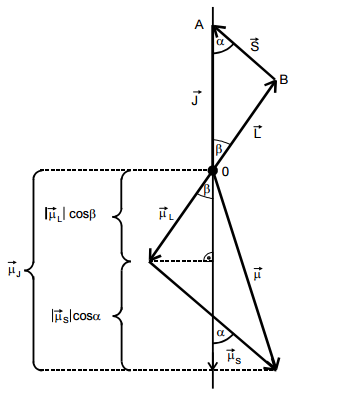
\includegraphics[width=0.3\textwidth]{winkel.png}
 \caption{Vektordiagramm der Drehimpulse einer Elektronenhülle und den resultierenden magnetischen Momenten.\cite{sample} }
 \label{fig:winkel}
 \end{figure}
Mit dem Cosinussatz und weiteren Umrechnung ergibt sich folgendes:
\begin{align}
 |\vec{\mu_\mathrm{J}}| \approx \mu_\mathrm{B} g_\mathrm{J} \sqrt{J(J+1)}.
\end{align}
Der Landé-Faktor $g_\mathrm{J}$ ist definiert durch:
\begin{align}
  g_\mathrm{J}=\frac{3J(J+1)+\left\{S(S+1)-L(L+1)\right\}}{2J(J+1)}.\label{eqn:lande}
\end{align}
Ein Quantenmechanischer Effekt ist die Richtungsquantelung,
die sagt aus, dass der Winkel zwischen äußerem Magnetfeld und
$|\vec{\mu_\mathrm{J}}|$  nicht beliebig sein kann, sondern $2J+1$
verschiedene Einstellungen. Diese Winkeleinstellungen legen potentielle Energien fest,
damit kann die Magnetisierung $\vec{M}$ berechnet werden und damit schließlich
die Suszeptibilität:
\begin{align}
  \Chi=\frac{\mu_0\mu_\mathrm{B}^2g_\mathrm{J}^2NJ(J+1)}{3kT}.\label{eqn:XT}
\end{align}
$N$ ist die Anzahl der Momente pro Volumeneinheit, $k$ ist die Bolzmann-Konstante und
$T$ die Temperatur. An dieser Formel ist auch die proportionalität zur $1/T$ zu erkennen.\\
Atome Seltener-Erd-Metalle besitzen einen stark ausgeprägten Paramagnetismus,
verantwortlich dafür sind die Elektronen der 4f-Schale. Die Anordnung der Elektronen dieser
Schale und damit der Gesamtdrehimpuls folgen den hundschen Regeln:
\begin{itemize}
  \item Die Spins $\vec{s}$ addieren sich zum maximalen Gesamtspin
   $\vec{S}=\sum s_i$, der nach dem Pauli-Prinzip möglich ist.
   \item Die Bahndrehimpulse $\vec{l}$ addieren sich zum maximalen Drehimpuls
   $\vec{L}=\sum l_i$, der nach Pauli-Prinzip und oberer Regel möglich ist.
   \item Der Gesamtdrehimpuls beträgt $|\vec{J}=\vec{L}-\vec{S}|$ wenn die
   Schale weniger als halb befüllt ist und $\vec{J}=\vec{L}+\vec{S}$ wenn die
   Schale mehr als halb befüllt ist.
\end{itemize}
Nach dem Pauli-Prinzip müssen sich alle Elektronen in einem Atom in mindestens
einer Quantenzahl unterscheiden.
